\documentclass[11pt,a4paper]{article}
\usepackage[margin=1in]{geometry}
\usepackage{booktabs}
\usepackage{graphicx}
\renewcommand{\thefigure}{S\arabic{figure}}
\renewcommand{\thetable}{S\arabic{table}}

\begin{document}

\begin{center}
\textbf{\Large Supplementary material}\\[0.5em]
\textbf{Semantic Identifiability under Band-Order Ambiguity in PlanetScope Landslide Segmentation}
\end{center}

\section*{Supplementary Method S1: documented CAS external check}

The executed code assigns eight CAS RGB subdatasets by a salted hash of the
region name. The only surviving protocol was corrected and first committed
after execution; it is therefore a post-execution record, not independently
verifiable prospective specification or preregistration. Development used Lombok,
Moxitaidi UAV-1m, Hokkaido, and Wenchuan; Palu was the sole validation region;
Mengdong, Moxi town UAV-1m, and Tiburon Peninsula PlanetScope were designated
evaluation regions. Wenchuan replaced Moxi town in development after one
loader-semantics access, before model fitting; neither predictions nor metrics
were inspected. The same three-channel zero-control residual-attention model
was trained with base or plain boundary loss for seeds 42, 43, and 44. Fixed
non-overlapping 128-pixel crops, optimization budget, augmentations, and
validation-only threshold grid were shared. The executed limits were 80 source
tiles per development region and 160 per validation/test region, each yielding
16 crops. The post-run record lists four quantitative conditions: at least
+1.5 boundary-F1 points, positive effects in all three held regions, F1
non-inferiority within one point, and non-negative F1 effects for at least two
seeds. Independent recomputation verified all 150 event metrics.
The observed event-macro changes were $-2.19$ F1 points and $-1.86$ boundary-F1
points; held-region boundary effects were $-0.39$, $-5.14$, and $-0.05$ points.

\begin{table}[htbp]
\centering
\caption{Paired plain-boundary minus base-loss effects by designated CAS region and
seed, in F1/boundary-F1 percentage points. The macro row averages the three
regions within each seed.}
\label{tab:s1}
\small
\begin{tabular}{lccc}
\toprule
Region & Seed 42 & Seed 43 & Seed 44 \\
\midrule
Mengdong & $-8.66/+1.54$ & $-2.40/-1.57$ & $+1.74/-1.15$ \\
Moxi town & $-12.73/-1.16$ & $+3.50/-10.69$ & $+0.13/-3.58$ \\
Tiburon Peninsula & $-9.88/-0.38$ & $+2.57/-0.24$ & $+5.99/+0.46$ \\
\midrule
Event macro & $-10.42/+0.00$ & $+1.22/-4.17$ & $+2.62/-1.42$ \\
\bottomrule
\end{tabular}

\end{table}

Only one of four quantitative conditions passed: two seeds had non-negative macro F1
effects. The mean boundary-F1 gain was below $+1.5$ points, not every held
region had a positive mean boundary effect, and mean F1 was below the
$-1$-point non-inferiority bound. A separate process condition required no
post-access code, threshold, or reporting-rule change; because the protocol
was first committed after execution, that condition is not independently
time-verifiable and is not counted as passed.

\section*{Supplementary Method S2: internally precommitted LRD stress test}

The protocol, code, 16-development/6-validation/6-protected EID split, crop
rule, outcomes, and four criteria were locally committed as
\texttt{97b107836a3737436b973adb28d0f5c5be6c3d63} before validation or
protected optical access, but no public third-party pre-access timestamp exists.
Each EID uses up to 64 coordinate-hashed
128-pixel crops from named POST1 Sentinel-2 B04/B03/B02 rasters and its mask.
Six zero-control models cross base/plain-boundary loss with seeds 42--44.
Checkpoints and validation thresholds were hashed before a protected-fetch
authorization was issued. Independent recomputation matched all 330 metrics.

All four frozen criteria fail, but validation maximum F1 is $0.008$--$0.151$
and 84.1\% of protected crops are empty. The frozen boundary effect is
$-24.10$ points; empty/empty scoring of zero gives $-0.15$, pooled scoring
$-4.92$, and a common 0.5 threshold $-0.55$. A family audit groups development
PH0003 with protected PH0001/PH0004, leaving four non-overlapping EIDs.
Accordingly the run is failed/indeterminate sensitivity evidence, not
confirmation.

\begin{table}[htbp]
\centering
\caption{Frozen LRD plain-boundary minus base-loss effects. EID rows
average seeds; seed rows average six protected EIDs.}
\label{tab:s2}
\small
\begin{tabular}{lrr}
\toprule
Unit & $\Delta$F1 (points) & $\Delta$BF1 (points) \\
\midrule
CA0002 & $-5.42$ & $-25.56$ \\
CN0002 & $+0.66$ & $-22.38$ \\
IR0002 & $+0.22$ & $-25.77$ \\
PH0001 & $-10.10$ & $-24.78$ \\
PH0004 & $-10.57$ & $-21.45$ \\
US0001 & $-3.18$ & $-24.64$ \\
\midrule
Seed 42 macro & $+0.98$ & $-77.19$ \\
Seed 43 macro & $-0.04$ & $-0.06$ \\
Seed 44 macro & $-15.13$ & $+4.96$ \\
\midrule
Across-seed macro & $-4.73$ & $-24.10$ \\
\bottomrule
\end{tabular}

\end{table}

\section*{Supplementary Method S3: authorized Sen12 stress test}

Sen12Landslides provides named Sentinel-2 B02/B03/B04/B08
variables and inventory labels. The public protocol evolved fail-closed before
model outcomes: v1 omitted official task membership; v2 exposed the
\texttt{usa\_puertorico}$\rightarrow$\texttt{usa} alias; v3 failed its
China-held-out development floor; v4 passed scientific floors but failed an
over-strict float32 reproduction check; and v5 was publicly locked
(\texttt{a4fc497}), fitted, and authorized (\texttt{3f39077}) before 1,889
selected files from ten protected inventories were extracted. Version 6 was a
public post-access execution correction: one Indonesia post-image SCL array
contained 255, outside official classes 0--11. The correction retains 255 in
histograms and excludes it only from descriptive cloud denominators; no file,
input, mask, endpoint, or condition changed. It was published before model
inference. One protected MASK count observed during diagnosis is disclosed.

Independent verification recomputed 420 primary metric cells, 294
high-confidence cells, all ten SCL summaries, and every registered condition.
Only condition 2 passed. The registered transformed-envelope check reports one
Kyrgyzstan overlap, whereas the native same-CRS pixel-edge rectangles only
share an edge and have zero positive-area overlap. The former fails the frozen
bar; the latter prevents interpreting that failure as demonstrated duplication.

\begin{table}[htbp]
\centering
\caption{Registered Sen12 cross-dataset recurrence conditions. Intervals are
inventory-bootstrap 95\% intervals. Contrast values are percentage points.}
\label{tab:s3}
\begin{tabular}{@{}p{0.22\textwidth}p{0.22\textwidth}p{0.36\textwidth}c@{}}
\toprule
Condition & Estimate & Registered requirement & Result \\
\midrule
Index attention -- raw F1 &
$+0.70$ [$+0.28,+1.16$] pt &
Upper 95\% bound $<+1.00$ pt & Fail \\
Index modulation -- plain F1 &
$-0.06$ [$-0.41,+0.26$] pt &
Upper 95\% bound $<+1.00$ pt & Pass \\
Plain-boundary F1 &
$+0.61$ [$-0.09,+1.32$] pt; 5/10 positive &
All control means $>0$; pooled lower bound $>0$; positive in at least 8/10 &
Fail \\
Absolute F1 &
Arm means $1.21$--$3.14\%$ F1 &
Every arm mean at least $10\%$ F1 & Fail \\
Spatial integrity &
1 transformed-envelope intersection &
Zero cross-inventory intersections & Fail \\
\bottomrule
\end{tabular}

\end{table}

Supplementary Table~S4 reports the detailed RGBN-candidate HR-GLDD operating
metrics underlying the compact main comparison.

\begin{table}[htbp]
\centering
\caption{Detailed RGBN-candidate HR-GLDD outcomes. Values are three-seed
mean (population standard deviation); thresholds are validation-selected.}
\label{tab:s4}
\footnotesize
\setlength{\tabcolsep}{5pt}
\begin{tabular}{@{}lrrr@{}}
\toprule
Configuration & F1 (\%) & Boundary F1 (\%) & Default FPR (\%) \\
\midrule
U-Net/base & 66.92 (0.68) & 49.62 (0.63) & 2.19 (0.06) \\
ResU-Net/base & 68.55 (0.56) & 52.93 (0.79) & 2.30 (0.08) \\
Attn-zero/base & 68.88 (0.58) & 53.17 (0.25) & 2.23 (0.03) \\
Attn-raw/base & 69.13 (0.28) & 53.15 (0.14) & 2.25 (0.07) \\
Attn-NDVI/base & 68.92 (0.49) & 52.83 (0.48) & 2.27 (0.08) \\
Attn-NDVI/plain-boundary & 70.12 (0.19) & 56.20 (0.33) & 2.50 (0.07) \\
Attn-zero/plain-boundary & 69.99 (0.52) & 56.04 (0.43) & 2.50 (0.08) \\
Attn-raw/plain-boundary & 70.19 (0.30) & 56.15 (0.41) & 2.50 (0.12) \\
Attn-NDVI/NDVI-boundary & 69.92 (0.28) & 56.29 (0.32) & 2.55 (0.11) \\
\bottomrule
\end{tabular}
\par\vspace{0.6em}
\begin{tabular}{@{}lrrr@{}}
\toprule
Configuration & Matched FPR (\%) & Matched precision (\%) & 10-m F1 (\%) \\
\midrule
U-Net/base & 2.19 (0.06) & 76.86 (0.55) & 61.84 (0.42) \\
ResU-Net/base & 1.99 (0.06) & 78.27 (0.20) & 64.22 (0.37) \\
Attn-zero/base & 1.98 (0.09) & 78.59 (0.56) & 63.71 (0.45) \\
Attn-raw/base & 1.98 (0.07) & 78.69 (0.41) & 63.92 (0.15) \\
Attn-NDVI/base & 2.01 (0.06) & 78.41 (0.26) & 64.11 (0.32) \\
Attn-NDVI/plain-boundary & 1.99 (0.06) & 78.60 (0.32) & 65.33 (0.32) \\
Attn-zero/plain-boundary & 1.97 (0.05) & 78.63 (0.16) & 65.35 (0.47) \\
Attn-raw/plain-boundary & 1.98 (0.08) & 78.74 (0.56) & 65.56 (0.12) \\
Attn-NDVI/NDVI-boundary & 2.00 (0.06) & 78.44 (0.32) & 65.36 (0.19) \\
\bottomrule
\end{tabular}

\end{table}

\begin{table}[htbp]
\centering
\caption{Semantic-identifiability certificate over the two metadata-consistent
HR-GLDD schemas. Envelopes span schema-specific descriptive mean contrasts;
they are not confidence intervals.}
\label{tab:s5}
\footnotesize
\setlength{\tabcolsep}{3.2pt}
\begin{tabular}{@{}lrrrl@{}}
\toprule
Contrast (points) & RGBN & BGRN & Envelope & Direction \\
\midrule
Index input vs raw, F1 & -0.01 & -0.21 & [-0.21, -0.01] & negative \\
Index vs plain loss, F1 & -0.41 & -0.33 & [-0.41, -0.33] & negative \\
Index vs plain loss, BF1 & +0.38 & -0.05 & [-0.05, +0.38] & unidentified \\
Plain boundary vs base, F1 & +0.96 & +1.13 & [+0.96, +1.13] & positive \\
\bottomrule
\end{tabular}

\end{table}

\begin{figure}[htbp]
\centering
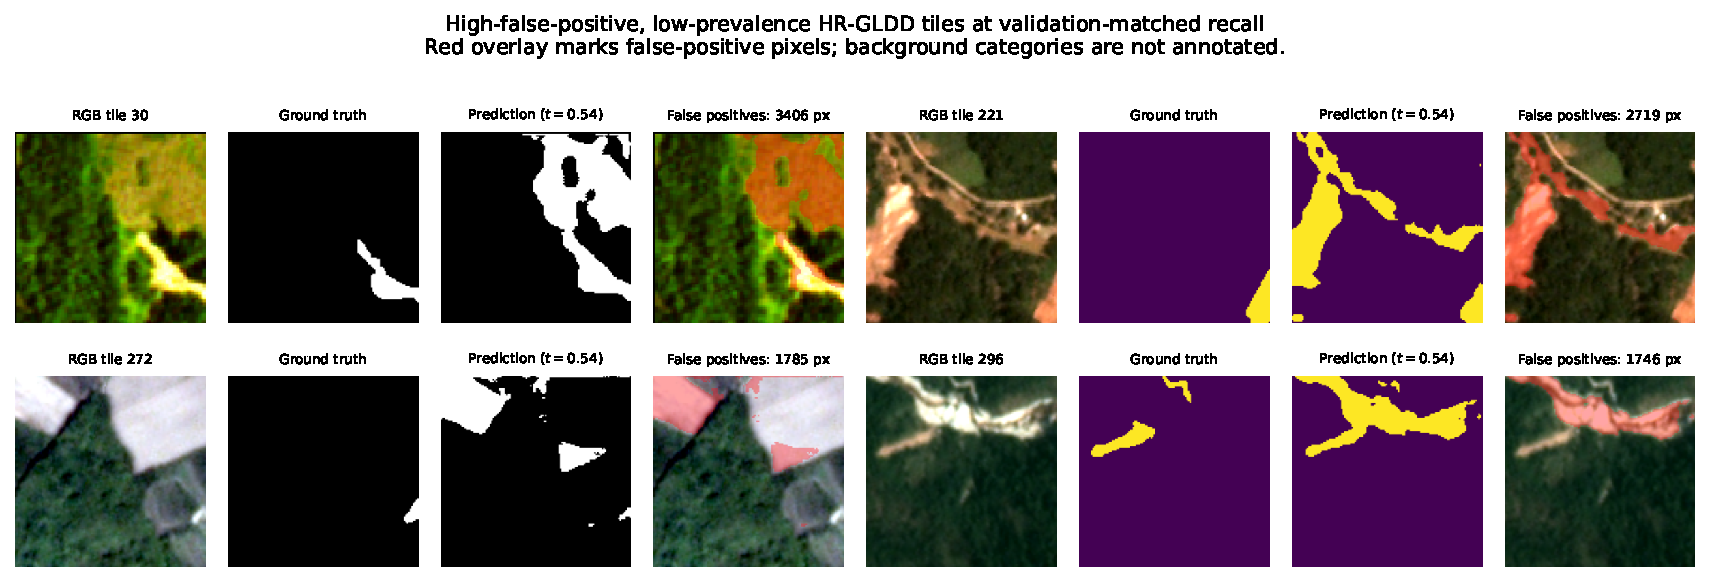
\includegraphics[width=\textwidth]{figures/fig_false_positive_atlas.pdf}
\caption{Four low-prevalence HR-GLDD test tiles with the largest false-positive counts for zero-control plus plain-boundary weighting at validation-matched recall (seed 42). Visible composites follow the official notebook's direct columns-0--2 display and are not band-order evidence. Red overlays denote false-positive pixels; background categories are not annotated.}
\label{fig:s1}
\end{figure}

\end{document}
